

\section{Architecture}

\subsection{Generator}

The ulimate aim of a Generative Adversarial Network is to train the Generator network to estimate an HR image for every LR image given as input.


\begin{figure}[h]
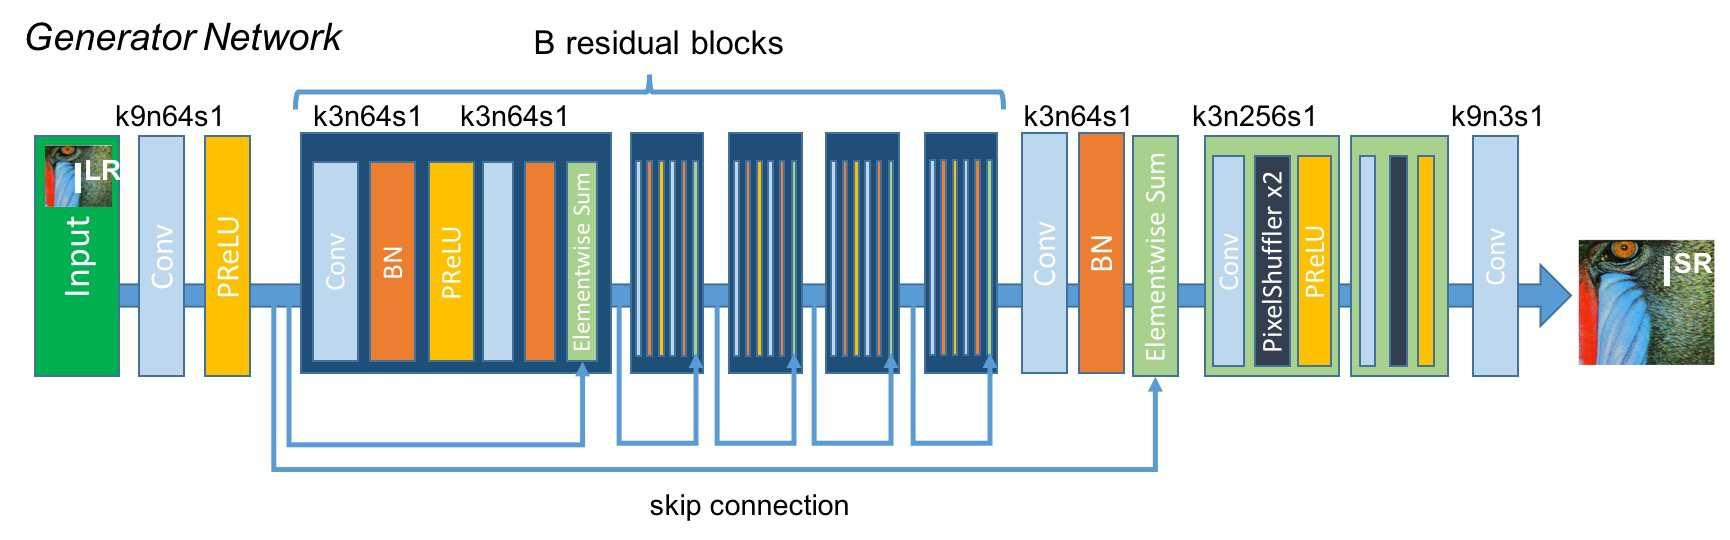
\includegraphics[scale=0.25]{ge}
\caption{Generator Network Architecture [3]}
\end{figure}


The Genertor Network G, is a very deep Network as illustrated in the figure. The input layer of the Generator network is a part of a convolutional neural network with a $9\times 9$ kernal size and has 64 feature maps. The convolution neural network uses Parameterised Rectified Linear Unit(PReLU) as activation function. 

The approximating linear components of the input using nonlinear activation function is too expensive. Hence Residual neural networks, which can asymptotically approximate complicated functions, are used. The working of residual neural networks can be said as, they explicitly approximate $F(x)-x$ rather than $F(x)$, where $x$ is its input. There are 16 blocks of Residual networks. Each having a convolution neural network, Batch Normalisation BN, activation function PReLU, which is followed by another convolutional nueral network and batch normalisation layers. The last layer of the residual block is an Elementwise sum layer which adds does the elementwise sum of output and input of the residual block. Both the convolution layers have $3\times 3$ kernals convolting with stride 1 producing 64 feature maps. The Entire stack of 16 residul blocks are followed by a convolutional network(k3n64s1), Batch normalisation layer and an Elementwise Sum layer. 

The resolution of the Image is increased by two blocks with a Convolution layer(k3n256s1), a Pixel shuffler($\times 2$) each. And is followed by the final layer  
being a convolutional network with $ 9\times 9 $ kernal and 3 feature maps.

\subsection{Discriminator}

The dicriminator network D, is trained to discriminate real High Resolution image from generated Super Resolved image. The architecture of the Discriminator network is shown in the image.

\begin{figure}[h]
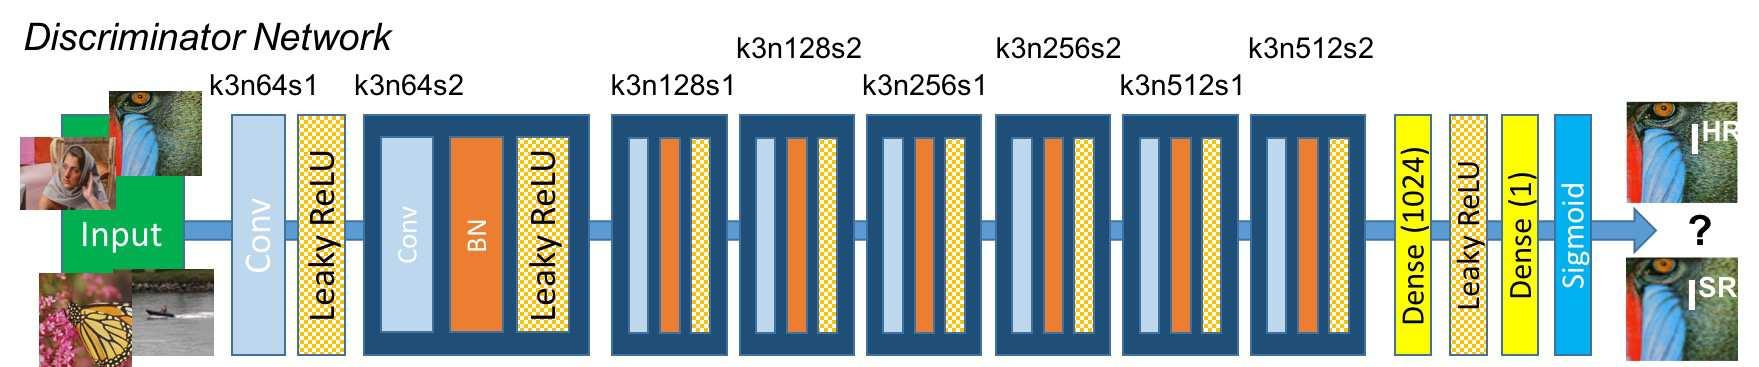
\includegraphics[scale=0.25]{dis}
\caption{Discriminator Network Architecture [3]}
\end{figure}

The input is received by a convolution neural network with a $3\times 3$ kernal and 64 feature maps convoluting with stride 1. It uses an activation function Leaky ReLU $(\alpha = 0.2)$. Maxpooling is avoided throughout the network.

Discriminator consists of eight such convolutional layers with an increase number of $ 3\times 3 $ filter kernels, becoming twice from 64 to 512. The architecture closely resembles that of the VGG networks. The layers convolute with stride 2 and 1 for alternate layers.

The stack of convolution layers with 512 feature map output is followed by two dense layers to serialise the feature maps. Finally a sigmoid activation function is applied to obtain the probability of the image for being SR or HR.
